\documentclass[a4paper]{article}
\usepackage{graphicx}
\usepackage{xcolor}
\usepackage{url}
\usepackage{outlines}
\usepackage{listings}
\usepackage{fontspec}
\usepackage{multicol}
\lstset{basicstyle=\ttfamily,
	showstringspaces=false,
	commentstyle=\color{blue},
	keywordstyle=\color{pink}
}
\lstset{emph={
	EXPOSE,RUN,FROM,CMD,nc,udp,http,docker},emphstyle=\color{purple}
}
\newcommand{\abc}{\hfill \break}
\newcommand{\ii}{\textit}
\usepackage{fancyhdr}
\usepackage{geometry}
% \usepackage{hyperref}
% \hypersetup{
% 	colorlink=true,
% 	linktoc=all,
% 	linkcolor=pink,
% }
\geometry{
	a4paper,
	total={170mm,257mm},
	left=20mm,
	top=20mm,
	bottom=39mm,
}

\setlength{\headheight}{82.70538pt}

\fancypagestyle{oida}{
	\fancyhf{}
	\fancyhead[L]{\fontsize{7.5}{7.5}htl donaustadt\\ Donaustadtstraße 45\\
		1220 Wien\\~\\ Abteilung: Informationstechnologie\\ 
	Schwerpunkt: Netzwerktechnik}
	\fancyhead[R]{
\includegraphics[scale=0.45]{images/logo.png}}

	\fancyfoot[L]{\today}
	\fancyfoot[C]{\jobname}
	\fancyfoot[R]{Seite: \thepage}
}

\begin{document}
\pagestyle{oida}
\section*{Configure Basic Router Settings}
\par\noindent\rule{\textwidth}{0.4pt}

Laboratory protocol
Configure Basic Router Settings

\begin{figure}[h]
	
\includegraphics[scale=0.2]{images/mika.jpeg}
	\centering
\end{figure}

\vspace*{\fill}
Subject:	NWT|ANGE

Class:	3AHITN

Name:	Stefan Fürst, Marcel Raichle

Group Name/Number: Dumm und Dümmer/7

Supervisor: 	ANGE

Exercise dates:	8.11.2024 29.11.2024 6.12.2024

Submission date: 12.12.2024


\newpage
\tableofcontents

\newpage

\section{Task definition}

In this exercise, it is required to set up a basic router configuration, which includes configuring SSH for remote access, securing all other login methods, and setting IP addresses.

\section{Summary}

This exercise is about configuring router settings and verifying network connectivity. It involves assigning IPv4 and IPv6 addresses, setting up SSH for remote access, and applying security measures such as passwords and login protocols. Connectivity is tested through pings and SSH access. Router information is retrieved using commands like \ii{show version} and \ii{show ip route}, while interface and IPv6 settings are examined. The exercise emphasizes router configuration, network security, and troubleshooting. \footnote{This summary was created with ChatGPT.}
\newpage

\section{Complete network topology of the exercise}
\begin{figure}[h]
	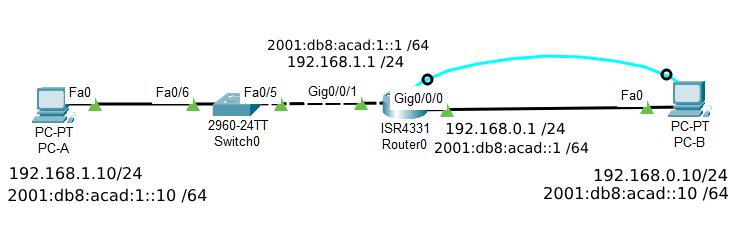
\includegraphics[scale=0.65]{images/nwtopology2.png}
	\centering
	\caption{Complete network topology of this exercise}
\end{figure}

\newpage

\section{Exercise Execution}
\subsection{Set Up the Topology and Initialize Devices}
This exercise was done in Cisco Packet Tracer and the devices were placed and wired using the automatic cabling type, as all the devices are Auto-MDIX compliant anyway.\abc
\begin{figure}[h]
	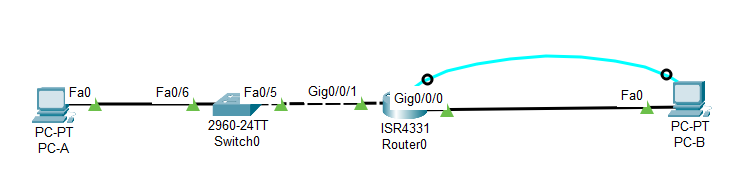
\includegraphics[scale=0.45]{images/nwtopology.png}
	\centering
	\caption{Network topology required for this exercise}
\end{figure}\abc
After that, everything was turned on and the router and switch were both iniliazised and reloaded.

\subsection{Configure Devices and Verify Connectivity}
\subsubsection{Configure the PC interfaces}
The IP addresses for both PCs have been set in the IP Configuration application.
\begin{figure}[h]
	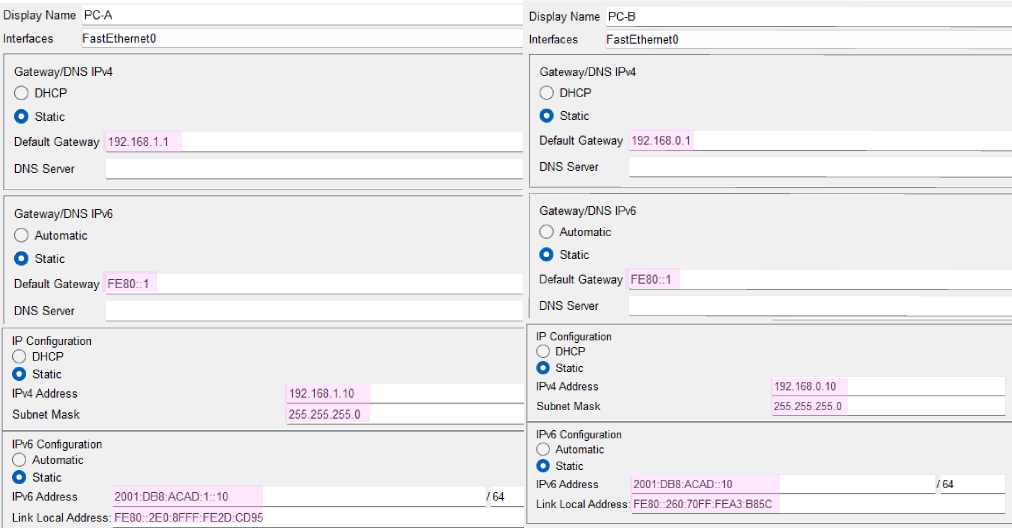
\includegraphics[scale=0.45]{images/pc-ipconf.png}
	\centering
	\caption{IP configuration for PC-A and PC-B}
\end{figure}
\newpage
\subsection{Configure the router}
To access the router's configuration mode, connect to the router through the console port and execute the \ii{en} and \ii{conf t} commands.\abc
The following basic settings are configured using the commands listed below:
\begin{lstlisting}[language=bash,
	keywordstyle=\color{black},
	rulecolor=\color{blue}]
#setting the hostname
hostname R1
#setting the domain name of the router
ip domain name ccna-lab.com
#disable DNS lookup on mistyped commands
no ip domain lookup
#encrypt plain text passwords
service password-encryption
#setting the minimum password length to 12 characters
security passwords min-length 12
\end{lstlisting}
To set up SSH for configuring the router over the network, first, a user must be created with the \ii{username SSHadmin secret 55Hadm!n2020} command, which creates a user named SSHadmin and sets an encrypted password.\abc
Once the user has been created, an RSA key pair needs to be generated using the \ii{crypto key generate rsa general-keys modulus 1024}\footnote{As this is done in Packet Tracer and the hardware in the lab is outdated, the keys are limited to 1024 bit length instead of the 4096 bit length that should be used in a production environment.} command.

\begin{figure}[h]
	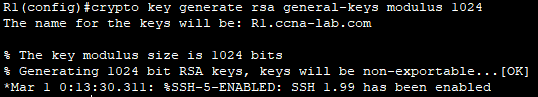
\includegraphics[scale=0.55]{images/keygen.png}
	\centering
	\caption{Key pair generation}
\end{figure}
\begin{lstlisting}[language=bash,
	keywordstyle=\color{black},
	rulecolor=\color{blue}]
#setting a password to enter EXEC mode
enable secret $cisco!PRIV*
line console 0
#setting password for console access
password $cisco!!CON*
#termination of the session after four minutes of inactivity
exec-timeout 4 0
#enabeling login 
login
\end{lstlisting}
\begin{figure}[h]
	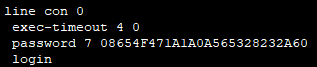
\includegraphics[scale=0.55]{images/line con0.png}
	\centering
	\caption{Viewing the configuration of VTY line 0}
\end{figure}
\begin{lstlisting}[language=bash,
	keywordstyle=\color{black},
	rulecolor=\color{blue}]
#entering the configuration for lines for vty lines 0 to 4
line vty 0 4
#setting a password to access the lines
password $cisco!!VTY*
#termination of the session after four minutes of inactivity
exec-timeout 4 0
#only allowing ssh connections
transport input ssh
#enabeling login using the local database
login local
\end{lstlisting}
\begin{figure}[h]
	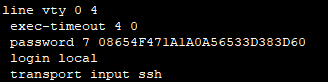
\includegraphics[scale=0.55]{images/votylines.png}
	\centering
	\caption{Viewing the configuration of VTY lines 0 4}
\end{figure}
\begin{lstlisting}[language=bash,
	keywordstyle=\color{black},
	rulecolor=\color{blue}]
#createing a banner to warn that unauthorized access is prohibited
banner motd $ unauthorized access is prohibited $
\end{lstlisting}
\begin{figure}[h]
	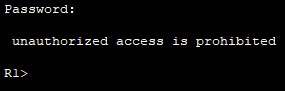
\includegraphics[scale=0.55]{images/banner.png}
	\centering
	\caption{Viewing the MOTD banner}
\end{figure}\abc

\begin{lstlisting}[language=bash,
	keywordstyle=\color{black},
	rulecolor=\color{blue}]
#enable ipv6 routing
ipv6 unicast-routing
#setting the ip addresses according to the addressing table
interface g0/0/0
ip address 192.168.0.1 255.255.255.0
ipv6 address fe80::1 link-local
ipv6 address 2001:db8:acad::1/64
no shutdown
exit
interface g0/0/1
ip address 192.168.1.1 255.255.255.0
ipv6 address fe80::1 link-local
ipv6 address 2001:db8:acad:1::1/64
no shutdown
exit
interface loopback0
ip address 10.0.0.1 255.255.255.0
ipv6 address fe80::1 link-local
ipv6 address 2001:db8:acad:2::1/64
no shutdown
exit
\end{lstlisting}
\newpage
\begin{figure}[h]
	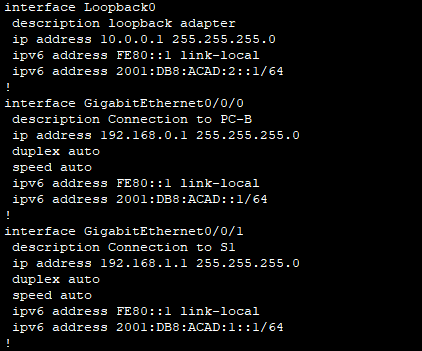
\includegraphics[scale=0.55]{images/showip.png}
	\centering
	\caption{Displaying the IP addresses set}
\end{figure}
\begin{lstlisting}[language=bash,
	keywordstyle=\color{black},
	rulecolor=\color{blue}]
#setting a timeout of 2 minutes after 3 failed login attempts in 60 seconds
login block-for 120 attempts 3 within 60
exit
#setting the clock
clock set 9:22:40 08 Nov 2024
\end{lstlisting}
\begin{figure}[h]
	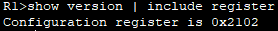
\includegraphics[scale=0.55]{images/showclock.png}
	\centering
	\caption{Display of current time}
\end{figure}\abc

\begin{lstlisting}[language=bash,
	keywordstyle=\color{black},
	rulecolor=\color{blue}]
#copying the current running-config to the startup-config
copy run start
\end{lstlisting}
If the router is reloaded before running this command, the running configuration will be lost, as the RAM is erased during a reload.
\newpage
\subsubsection{Verify network connectivity}
To test if everything was configured appropriately, PC-B will be pinged from PC-A to check if they can communicate.
\begin{figure}[h]
	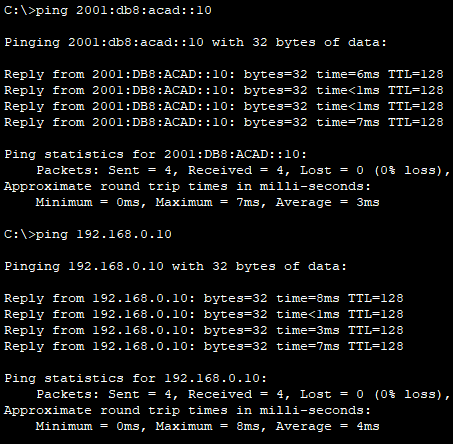
\includegraphics[scale=0.45]{images/pingpcb.png}
	\centering
	\caption{Pinging PC-B from PC-A}
\end{figure}\abc
Next, the SSH connection will be tested by connecting from PC-A to the router using its IPv4 and IPv6 addresses on the loopback interface.
\begin{figure}[h]
	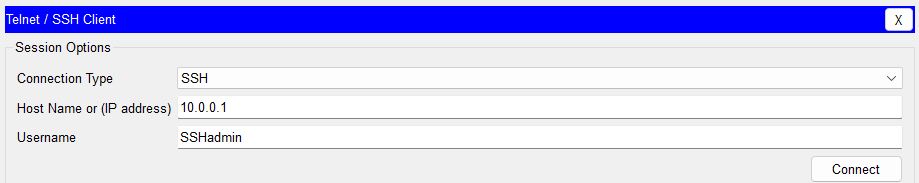
\includegraphics[scale=0.45]{images/ipv4ssh.png}
	\centering
	\caption{Connecting to the router via IPv4 using ssh}
\end{figure}\abc
\begin{figure}[h]
	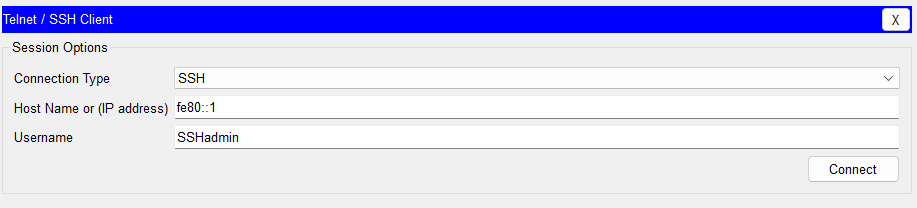
\includegraphics[scale=0.45]{images/ipv6ssh.png}
	\centering
	\caption{Connecting to the router via IPv6 using ssh}
\end{figure}\abc
\begin{figure}[h]
	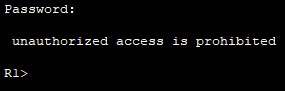
\includegraphics[scale=0.55]{images/banner.png}
	\centering
	\caption{Working login}
\end{figure}\abc
The Telnet protocol is considered a security risk because it is not encrypted, meaning that the entire session can be seen in clear text, allowing passwords to be easily exposed using a packet sniffer.
\subsection{Display Router Information}
\subsubsection{Retrieve important hardware and software information.}
The \ii{show version} command displays information about the hardware and software running on the router.
\begin{figure}[h]
	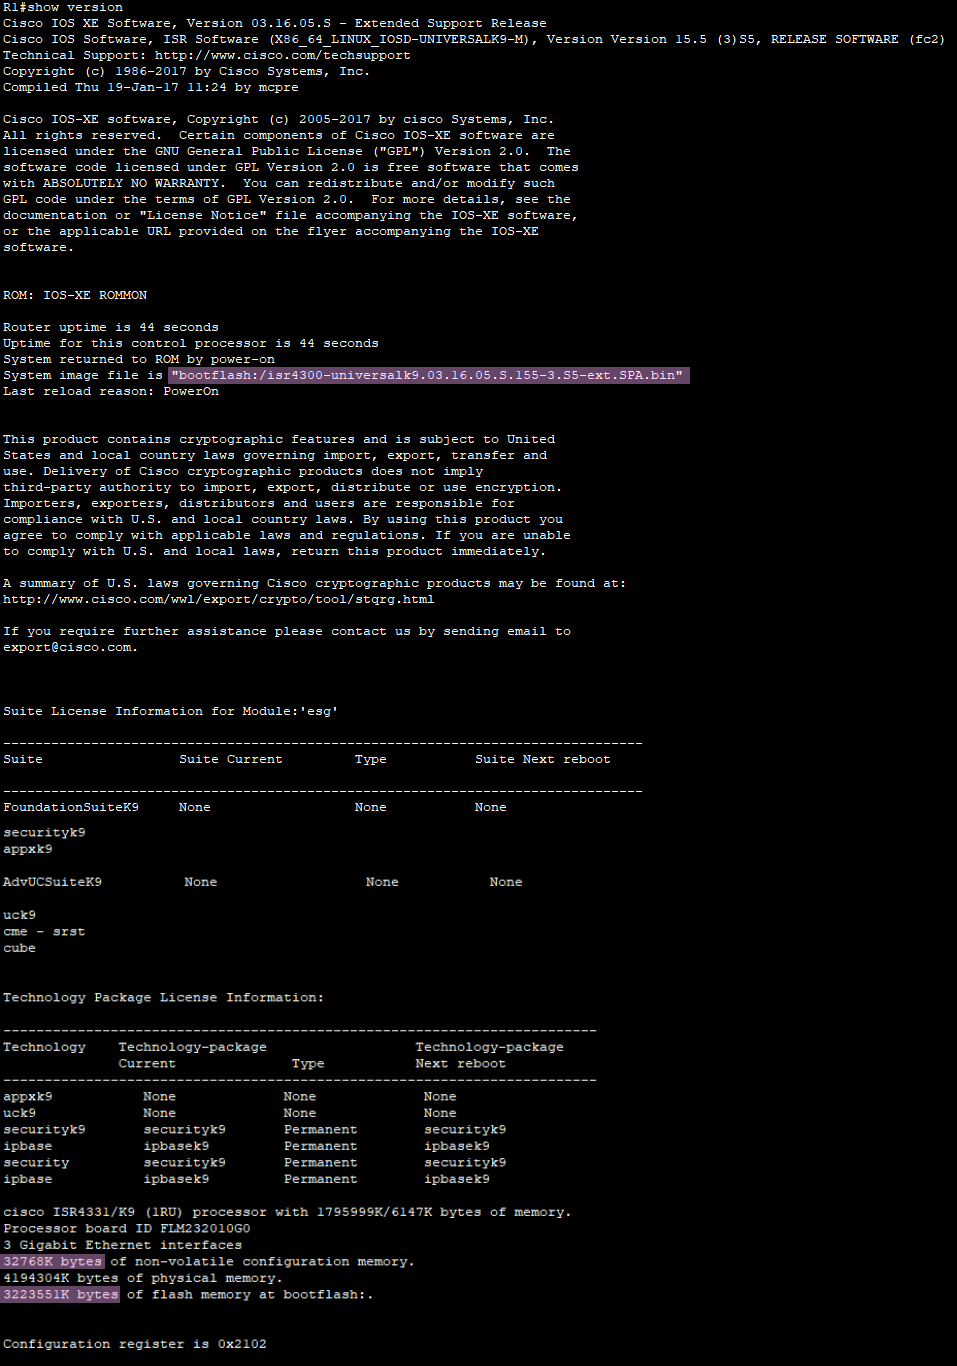
\includegraphics[scale=0.30]{images/showversion.png}
	\centering
	\caption{Displaying information about the hardware and software}
\end{figure}\abc
The name of the IOS image is \ii{isr4300-universalk9.03.16.05.S.155.3.S5-ext.SPA.bin}, and the router has 32 MB of NVRAM and 3.07 GB of flash memory.\newpage\abc
Since the output of this command is long and can be difficult to navigate, it can be filtered by piping the command and using the \ii{include} keyword with the desired search term.
\begin{figure}[h]
	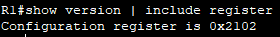
\includegraphics[scale=0.60]{images/grep.png}
	\centering
	\caption{Filtering the output of the show version command to show only the register}
\end{figure}\abc
The register is \ii{0x2142}, which means that the router will undergo the normal boot process: it will load the IOS image from flash memory and load the startup configuration from NVRAM if one is present.\abc
\subsubsection{Display the startup configuration}
The startup configuration is shown with the \ii{show startup-config} command, and due to the \ii{service password-encryption} command, the passwords are displayed in an encrypted form.
\begin{figure}[h]
	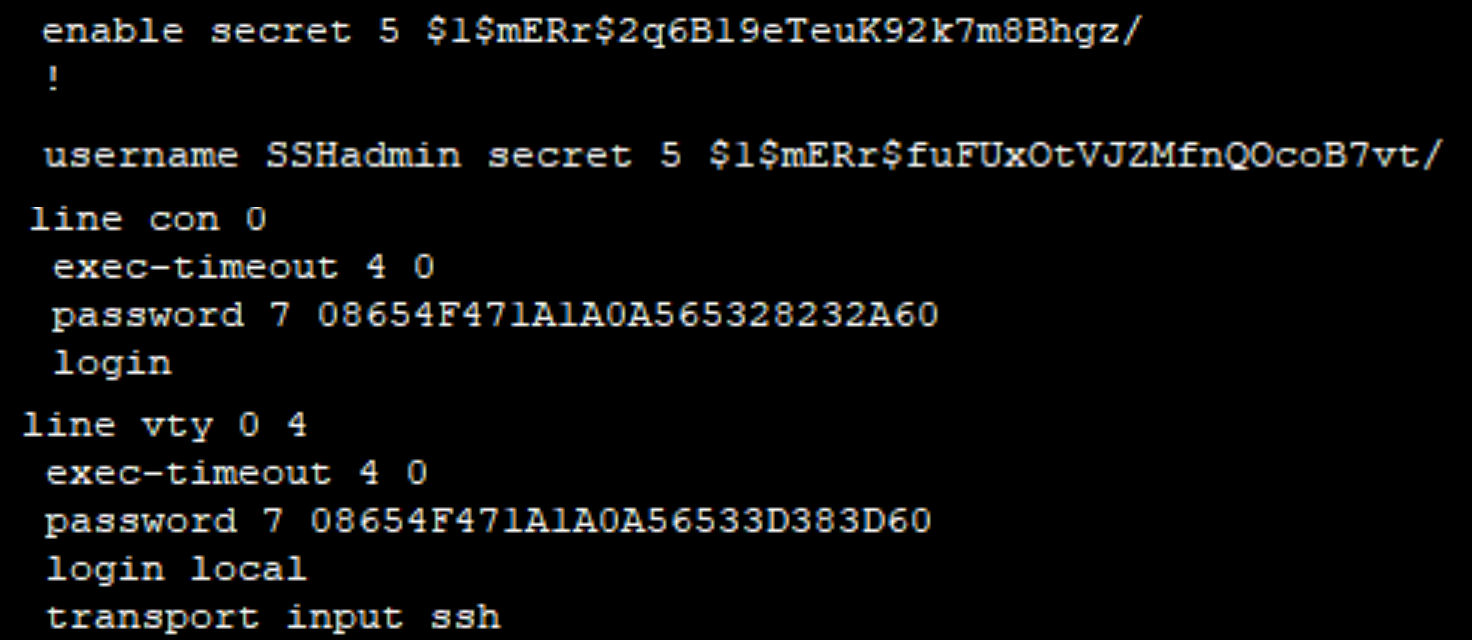
\includegraphics[scale=0.20]{images/passwords.png}
	\centering
	\caption{Passwords displayed in encrypted form}
\end{figure}\abc
Like with any other command, the output can be piped and filtered to show only specific sections. In this case, it is filtered to display only the VTY section of the startup configuration.\footnote{In Cisco Packet Tracer, piping the output of the show run command doesn't work, so this screenshot was created using Photoshop. The output was taken from the show startup-config command without any filtering and edited to appear as if it was filtered.}
\begin{figure}[h]
	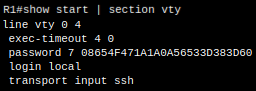
\includegraphics[scale=0.60]{images/clueless.png}
	\centering
	\caption{Filtering the output of show run to only display the VTY section}
\end{figure}\abc
\newpage
\subsubsection{Display the routing table on the router}
The routing table of the router can be displayed with the \ii{show ip route} command.
\begin{figure}[h]
	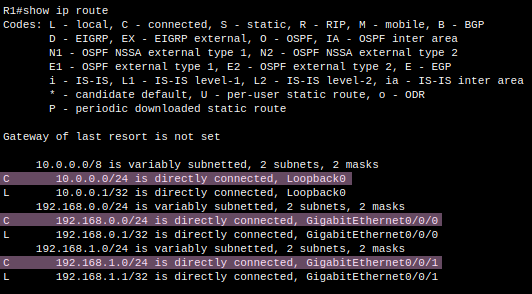
\includegraphics[scale=0.40]{images/show ip route.png}
	\centering
	\caption{Displaying the ip routes}
\end{figure}\abc
The \ii{C} code is used in the routing table to indicate a directly connected network, which corresponds to three entries in the routing table.
\subsubsection{Display a summary list of the interfaces on the router}
The IPv4 configuration of the interfaces is displayed with the \ii{show ip interface brief} command.
\begin{figure}[h]
	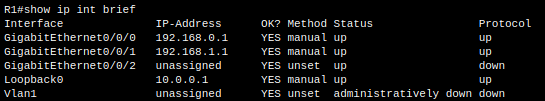
\includegraphics[scale=0.40]{images/showipintbrief.png}
	\centering
	\caption{Displaying a summary of the IPv4 configuration of interfaces}
\end{figure}\abc
The \ii{no shutdown} command is used to change the Ethernet ports from administratively down to up.\abc
The IPv6 configuration of the interfaces is displayed with the \ii{show ipv6 interface brief} command.
\begin{figure}[h]
	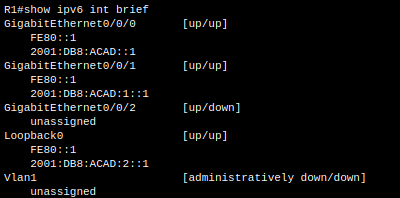
\includegraphics[scale=0.40]{images/showipv6intbrief.png}
	\centering
	\caption{Displaying a summary of the IPv6 configuration of interfaces}
\end{figure}\abc
The \ii{[up/up]} status indicates the Layer 1 and Layer 2 status of the interface and does not provide information about Layer 3.\newpage\abc
After changing the IPv6 configuration of PC-B to Automatic, the active configuration can be viewed in the command prompt with the \ii{ipconfig} command.
\begin{figure}[h]
	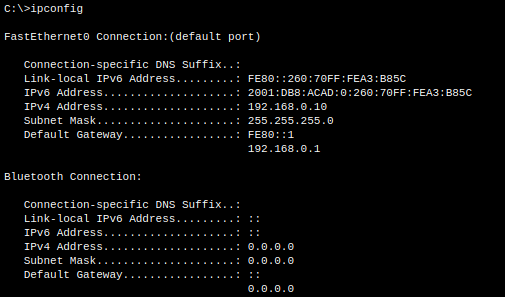
\includegraphics[scale=0.40]{images/ipconf.png}
	\centering
	\caption{Displaying the IP configuration of PC-B after setting the IPv6 configuration to automatic}
\end{figure}\abc
PC-B was assigned \ii{2001:DB8:ACAD:0:260:70FF:FEA3:B85C} as its address and \ii{FE80::1} as the default gateway.\abc
After pinging both the default gateway's link-local and IPv6 unicast addresses, it shows that both were successful, and the automatic configuration worked.
\begin{figure}[h]
	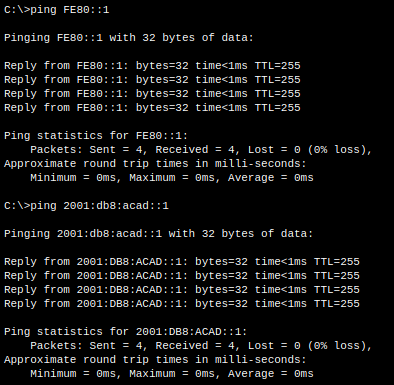
\includegraphics[scale=0.40]{images/pinging.png}
	\centering
	\caption{Pinging both the default gateway link local and IPv6 unicast address}
\end{figure}\abc
\subsection{Reflection Questions}
\begin{enumerate}
	\item In researching a network connectivity issue, a technician suspects that an interface was not enabled. What show command could the technician use to troubleshoot this issue?	
	\begin{enumerate}
		\item To check if an interface is not enabled, either the \ii{show interface brief} or \ii{show running-config/startup-config} command can be used. 
	\end{enumerate}
	\item In researching a network connectivity issue, a technician suspects that an interface was assigned an incorrect subnet mask. What show command could the technician use to troubleshoot this issue?
	\begin{enumerate}
		\item To check if an interface is assigned the wrong subnet mask, either the \ii{show protocols} or \ii{show running-config/startup-config} command can be used.
	\end{enumerate}
\end{enumerate}
\newpage
\section{Complete configuration files}
\begin{multicols}{2}
\begin{lstlisting}[language=bash,
	keywordstyle=\color{black},
	rulecolor=\color{blue}]
Current configuration : 1613 bytes
!
version 15.4
no service timestamps log datetime msec
no service timestamps debug datetime msec
service password-encryption
security passwords min-length 12
!
hostname R1
!
login block-for 120 attempts 3 within 60
!
enable secret 5\ 
$1$mERr$2q6B19eTeuK92k7m8Bhgz/
!
no ip cef
ipv6 unicast-routing
!
no ipv6 cef
!
username SSHadmin secret 5 \
$1$mERr$fuFUxOtVJZMfnQOcoB7vt/
!
no ip domain-lookup
ip domain-name ccna-lab.com
!
spanning-tree mode pvst
!
interface Loopback0
 description loopback adapter
 ip address 10.0.0.1 255.255.255.0
 ipv6 address FE80::1 link-local
 ipv6 address 2001:DB8:ACAD:2::1/64
!
interface GigabitEthernet0/0/0
 description Connection to PC-B
 ip address 192.168.0.1 255.255.255.0
 duplex auto
 speed auto
 ipv6 address FE80::1 link-local
 ipv6 address 2001:DB8:ACAD::1/64
!
interface GigabitEthernet0/0/1
 description Connection to S1
 ip address 192.168.1.1 255.255.255.0
 duplex auto
 speed auto
 ipv6 address FE80::1 link-local
 ipv6 address 2001:DB8:ACAD:1::1/64
!
interface GigabitEthernet0/0/2
 no ip address
 duplex auto
 speed auto
!
interface Vlan1
 no ip address
 shutdown
!
router rip
!
ip classless
!
ip flow-export version 9
!
ip access-list extended sl_def_acl
 deny tcp any any eq telnet
 deny tcp any any eq www
 deny tcp any any eq 22
 permit tcp any any eq 22
!
banner motd \
$ unauthorized access is prohibited $
!
line con 0
 exec-timeout 4 0
 password 7 08654F471A1A0A565328232A60
 login
!
line aux 0
!
line vty 0 4
 exec-timeout 4 0
 password 7 08654F471A1A0A56533D383D60
 login local
 transport input ssh
!
end
\end{lstlisting}
\end{multicols}
\newpage
\section{List of figures}

\listoffigures

\end{document}
